\documentclass{article}

% NeurIPS 2026 Evaluations & Datasets Track, single-blind (nonanonymous).
% ConstellationBench is a publicly released dataset; dataset-focused submissions
% in E&D are allowed to opt for single-blind so reviewers can inspect hosted code/data.
\usepackage[eandd, nonanonymous]{neurips_2026}

\usepackage[utf8]{inputenc}
\usepackage[T1]{fontenc}
\usepackage{hyperref}
\usepackage{url}
\usepackage{booktabs}
\usepackage{amsmath}
\usepackage{amsfonts}
\usepackage{amssymb}
\usepackage{nicefrac}
\usepackage{microtype}
\usepackage{xcolor}
\usepackage{graphicx}

\title{ConstellationBench and the Non-Separability Index: Measuring Behavioral Compression Under Preference Aggregation in 22 Frontier Language Models}

\author{%
  Zachary Holwerda \\
  Airlock Labs \\
  Detroit, MI \\
  \texttt{zac@airlocklabs.io} \\
}

\begin{document}

\maketitle

\begin{abstract}
We release ConstellationBench, a behavioral evaluation dataset of 22 language models across four architecture families (dense, MoE, Mamba-hybrid, hybrid-linear-attention), evaluated on seven DECF-based behavioral benchmarks across 22{,}200+ scored responses at approximately \$115 total API cost. We introduce the Non-Separability Index (NSI), a bivector-valued metric $S_M = \alpha_M \cdot 4 w_a w_b$ decomposing model response geometry into plane retention ($\alpha_M$) and balance between target and adversarial poles ($w_a, w_b$). Applied to a preregistered 10-model subset across five scenarios (750 cached responses, SHA-256-pinned lexicon, five locks frozen before collection), NSI is an independent axis of behavioral quality: Spearman $\rho = 0.018$ between $S_M$ and scalar persona fidelity on the same transcripts, with three rank inversions in the top five --- a Strong verdict on the preregistered independence gate. Heavier-RLHF frontier models exhibit systematically lower $S_M$ under adversarial pressure than lighter-alignment budget and MoE models --- the RLHF paradox visible in bivector space, consistent with the covariance-amplification mechanism of \citet{shapira2026rlhf}. We report partial failure on lexicon-perturbation robustness (Kendall $\tau = 0.200$ minimum, below the preregistered $0.7$ threshold) and a preregistered null on scenario-aware routing uplift ($\Delta = -0.006$, with a $+0.233$ oracle-to-static gap indicating query-level headroom). All artifacts release with Croissant metadata at \url{https://huggingface.co/datasets/AirlockLabs/constellation-bench}.
\end{abstract}

% =============================================================================
\section{Introduction}
\label{sec:intro}

The AI industry evaluates large language models along three axes: capability, cost, and speed. Every widely-cited benchmark --- MMLU \citep{hendrycks2021measuring}, HumanEval \citep{chen2021evaluating}, GPQA \citep{rein2023gpqa}, and their descendants --- measures what a model can \emph{do}. An increasing class of deployed systems, however, depends less on task completion than on \emph{behavioral consistency}: customer-service agents, tutors, coaches, creative collaborators, clinical triage assistants, and companion applications require the model to sustain a distinct behavioral identity across multi-turn conversations, under adversarial pressure, and in commercially adversarial contexts. For these deployments the model \emph{is} the character. A system that produces correct answers but cannot hold voice differentiation between a cautious guardian persona and a bold strategist persona is functionally unusable regardless of its reasoning score.

This gap is not merely a missing benchmark. It is a methodological limit of the dominant alignment paradigm. Contemporary frontier models are shaped primarily through reinforcement learning from human feedback \citep{christiano2017deep, ouyang2022training, bai2022constitutional} or direct-preference variants thereof, pipelines whose load-bearing assumption --- a scalar reward aggregated across heterogeneous raters via a Bradley-Terry model --- was validated in game-like domains with well-defined ground-truth outcomes. In open-ended conversational deployments, the ground-truth assumption does not hold: heterogeneous user populations do not share a preference the aggregation can converge to. The same pairwise comparison is evaluated differently by raters of different behavioral profiles, demographic groups, and task intents, and averaging across the disagreement discards the information a deployed router would need to serve any specific user well. Recent work formalizes this directly: \citet{shapira2026rlhf} prove a covariance-based mechanism linking biased preference data to sycophantic policy drift, \citet{kirk2024understanding} document the resulting behavioral-diversity collapse, and \citet{santurkar2023whose} show that the surviving distribution reflects narrow demographic slices. \citet{casper2023open} catalogs this and $\approx$35 adjacent open problems without proposing a technical successor; we argue here that the missing instrument is a measurement apparatus that quantifies the geometric structure the aggregation is throwing away.

\textbf{Contributions.} This paper makes three. First, as a dataset contribution, we release \emph{ConstellationBench}, a behavioral evaluation corpus of 22 language models across four architecture families (dense, Mixture-of-Experts, Mamba-Transformer hybrid, hybrid-linear-attention) spanning seven preregistered behavioral benchmarks at 22{,}200+ scored responses (\S\ref{sec:dataset}). Second, as a measurement contribution, we introduce the \emph{Non-Separability Index (NSI)}, a bivector-valued metric $S_M = \alpha_M \cdot 4 w_a w_b$ that decomposes a model response's geometric relationship to a preregistered target behavioral pole and a preregistered adversarial pole, quantifying both \emph{plane retention} ($\alpha_M$) and \emph{pole balance} ($w_a, w_b$) (\S\ref{sec:nsi}). Third, as an empirical study, we report a preregistered 10-model $\times$ 5-scenario application of NSI yielding a Strong verdict on the preregistered independence gate (Spearman $\rho = 0.018$ between $S_M$ and same-substrate scalar persona fidelity across the 10-model slate, three top-five rank inversions), an honestly-reported partial failure on lexicon-perturbation robustness, a null on scenario-aware routing uplift with substantial oracle-to-static headroom, and an architecture-dependent behavioral ceiling in which MoE models dominate performance layers while Dense models dominate depth layers (\S\ref{sec:empirical}).

We frame this work as a continuation, not a repudiation, of the preference-aggregation line of research. The method of \citet{christiano2017deep} established scalar-reward-from-preferences as a tractable alignment signal in Atari and MuJoCo, domains where trajectories have well-defined ground-truth outcomes humans can noisily rate. In open-ended conversational deployments the ground-truth assumption does not hold, and the authors' own 2017 reward-hacking concern compounds at model scales six orders of magnitude larger than the original setting. Our contribution is the dataset and measurement apparatus for quantifying what the aggregation discards; the architectural response is developed in a companion paper and deferred here (\S\ref{sec:future}).

% =============================================================================
\section{Related Work}
\label{sec:related}
% Page budget: 1.0
% Subsections per outline:
%   \S 2.1 Behavioral evaluation of LLMs
%   \S 2.2 Preference learning and its limits (includes Christiano touchpoint 2)
%   \S 2.3 Routing and cascading literature (Table 1 positioning NSI)
%   \S 2.4 Geometric framing precedents (brief; full theory in App. A)

\subsection{Behavioral evaluation of large language models}
The dominant LLM evaluation paradigm measures task performance: MMLU \citep{hendrycks2021measuring} tests knowledge breadth, HumanEval \citep{chen2021evaluating} measures code generation, GPQA \citep{rein2023gpqa} probes graduate-level scientific reasoning, and holistic frameworks such as HELM extend the same scalar-task posture across multiple dimensions. Persona- and character-consistency literature \citep{sharma2024sycophancy, perez2022discovering} moves closer to behavioral evaluation but typically measures consistency as a scalar property of surface agreement rather than as structure preserved under adversarial pressure. Psychometric applications to LLMs --- administering Big Five inventories and similar instruments to frontier models --- treat the model as a subject to be profiled; we invert that posture and treat the psychometric framework as a scoring rubric for evaluating how faithfully the model \emph{performs} a specified behavioral profile.

\subsection{Preference learning and its limits}
\label{sec:related:rlhf}
The method of \citet{christiano2017deep} is the direct ancestor of modern RLHF pipelines. Its Bradley-Terry scalarization was appropriate for game-like trajectories with well-defined outcomes (Atari, MuJoCo) and did not carry the ground-truth assumption forward to open-ended language. \citet{kirk2024understanding} document the downstream compression with a controlled SFT vs. reward-modeling vs. RLHF comparison: RLHF systematically decreases per-input diversity across syntactic, semantic, and entailment metrics, and KL-regularization tuning does not recover it. \citet{santurkar2023whose} extend the finding along demographic axes, showing the surviving distribution reflects a narrow slice of the raters. \citet{shapira2026rlhf} prove the amplification mechanism formally: a covariance-based result linking biased preference data to sycophantic policy drift, independent of KL strength. \citet{casper2023open} catalog $\approx$35 open problems of which preference heterogeneity, reward misspecification, and mode collapse are three, noting that no scalar reward can faithfully aggregate heterogeneous values. NSI is the orthogonal geometric measurement showing that the compression is bivector-structured: scalar-reward optimization does not merely narrow the response distribution, it flattens an oriented plane spanned by the target behavioral pole and the adversarial pull.

\subsection{Preference routing and cascading}
Inference-time routing between LLMs is an active frontier. \citet{ong2024routellm} train routers on preference data to navigate the quality--cost tradeoff between frontier and budget models; \citet{ding2024hybrid} route on query-difficulty scores; \citet{dekoninck2024cascade} unify cascading policies. These approaches differ from NSI-motivated routing on three axes: (i) their optimization objectives are scalar quality, cost, and latency, not behavioral non-separability; (ii) their input signals are query features and historical model performance, not the user--model interaction's geometric decomposition; (iii) their scope is dyadic query-to-model selection, not the triadic user--router--provider structure that heterogeneous deployments require. We position NSI as an orthogonal signal, combinable with existing quality--cost--latency routers as a constraint on the selection space rather than a replacement for them. The Workload-Router-Pool framework \citep{wrp2026} and the distributional-AGI / patchwork view \citep{patchworkagi2025} provide the deployment-systems context into which NSI plugs as a missing router-layer observable. \citet{chakraborty2024maxmin} attack the same heterogeneity problem from the reward-model side via a maxmin multi-objective formulation; our response is to leave the reward model behind and measure the consequence of its aggregation at inference time.

\subsection{Social-choice and geometric precedents}
The impossibility results of \citet{arrow1950difficulty} and \citet{sen1970collective} establish that no single scalar social-welfare function can aggregate individual preferences under reasonable constraints. RLHF's core operation is exactly that aggregation; the scalar-reward paradigm imports the aggregation problem without inheriting the seven-decade literature on its limits, a tension \citet{bakker2022finetuning} surface explicitly in their consensus-statement work. The cognitive-science literature on reference-dependent preferences \citep{kahneman1979prospect} reinforces the point: even within-rater preferences are not total orderings. The broader complex-systems tradition, following \citet{kauffman1993origins}, establishes that emergence is a graph-topology property rather than a node-intrinsic one --- intelligence in biological and social systems lives in the connective tissue between elements, not in the elements themselves. On the geometric side, the Geometric Algebra Transformer \citep{brehmer2023geometric} establishes architectural legitimacy for bivector-preserving attention in deployed models; Integrated Information Theory's $\Phi$ \citep{oizumi2014phenomenology} provides the closest methodological precedent to NSI by measuring irreducible relational structure. Contemporaneously with this work, the JEPA line of world-model research \citep{balestriero2025lejepa, maes2026leworldmodel} addresses representation collapse in compact latent spaces via random-projection distribution matching (Cram{\'e}r-Wold decomposition over unit-norm projections) --- structurally parallel to the bivector-preservation argument of \S\ref{sec:nsi} and complementary as a candidate regularizer for the behavior-aware DECF embedding direction of \S\ref{sec:future}. Full theoretical framing --- including the connection to biological routing mechanisms that demix heterogeneous signals at the point of use rather than aggregate them at source --- is deferred to Appendix A.

% =============================================================================
\section{ConstellationBench Dataset}
\label{sec:dataset}
% Page budget: 1.5
% Subsections per outline:
%   \S 3.1 DECF framework
%   \S 3.2 The 7 benchmarks
%   \S 3.3 Signal-word scoring methodology
%   \S 3.4 Experimental setup
%   \S 3.5 Dataset release

\subsection{The DECF behavioral framework}
\label{sec:dataset:decf}
DECF adapts the Predictive Index, a psychometric instrument validated across millions of human assessments, to language-model evaluation. It measures four orthogonal behavioral drives on a $0$--$10$ scale:
\textbf{D (Dominance)} --- assertiveness, directive language, action-bias;
\textbf{E (Extraversion)} --- social energy, enthusiasm, group-orientation;
\textbf{C (Patience)} --- stability, methodical pacing, deliberation;
\textbf{F (Formality)} --- structure, precision, procedural compliance.
A DECF profile is a four-tuple $(d, e, c, f) \in \{0, 1, \ldots, 10\}^4$ with thresholds high $\geq 7$, low $\leq 3$, middle $= 4$--$6$. We define 17 named profiles spanning a representative coverage of the four-dimensional space (Maverick $(10, 8, 1, 1)$, Guardian $(3, 3, 9, 8)$, Promoter $(7, 10, 2, 2)$, Specialist $(2, 2, 9, 10)$, Collaborator $(3, 8, 7, 3)$, and 12 others), clustered into three meta-archetypes: \emph{Drivers} (high-D, distinctive voice), \emph{Enforcers} (high-C/F, hold through structure), and \emph{Interpreters} (balanced, hardest to differentiate from baseline). The full 17-profile roster with drive specifications is versioned in \texttt{data/personas/profiles.json}.

\subsection{Seven behavioral benchmarks}
\label{sec:dataset:benchmarks}
ConstellationBench comprises seven benchmarks, each evaluating a distinct axis of behavioral fidelity under deployment-realistic conditions.
\textbf{OttoTau} (policy enforcement $+$ epistemic spine): 20 multi-turn scenarios with adversarial pressure, scoring position-hold rate across 3--5 turn challenges.
\textbf{PersonaFidelity} (voice differentiation): 17 DECF profiles $\times$ 10 business-neutral prompts scored by DECF signal-word matching.
\textbf{SessionFidelity} (context recall without hallucination): 10 synthetic session summaries with embedded facts, 5 probe questions each.
\textbf{ColdRead} (drive inference): model infers user DECF profile from minimal text input across three signal-richness levels.
\textbf{VoiceDrift} (persona stability over time): 6 personas $\times$ 10-turn conversations with per-turn signal-density scoring.
\textbf{CostPerLifecycle} (economic efficiency): 4-stage task lifecycle with total API cost benchmarked against competitor pricing.
\textbf{Bench Core} (council deliberation): 30 queries $\times$ 4 personas per council with weighted composite scoring across persona adherence, deliberation diversity, response quality, and JSON compliance. Full benchmark specifications, prompt templates, and scoring rubrics are documented in the accompanying dataset documentation.

\subsection{Signal-word scoring}
\label{sec:dataset:scoring}
Persona fidelity is scored by matching drive-appropriate signal words in model output against the target DECF profile. For each drive we maintain HIGH and LOW signal-word sets (89 words total across 8 sets); the dictionary is versioned at \texttt{data/signal-words/decf-signals.json} with SHA-256 \texttt{a7b99e35d916\ldots}. Given a response text and a drive $X$ with target value $v$ and observed high-signal ratio $r = h/(h + l)$, the score is
\[
s_X = \begin{cases}
r & \text{if } v \geq 7, \\
1 - r & \text{if } v \leq 3, \\
0.5 + 0.5(r - 0.5) & \text{if } 4 \leq v \leq 6,
\end{cases}
\]
and the composite fidelity is $F = \tfrac{1}{4}\sum_{d \in \{D,E,C,F\}} s_d$. The scoring is deterministic, reproducible from the cached transcripts, and acknowledged as a lexical rather than semantic approximation (\S\ref{sec:discussion}). We report lexicon-perturbation robustness explicitly (\S\ref{sec:empirical}) rather than claim substrate-invariance.

\subsection{Experimental setup and scale}
\label{sec:dataset:setup}
We evaluate 22 models spanning four architecture families and four cost tiers, all accessed via the OpenRouter API for uniform inference conditions. The March 2026 baseline covers 15 models (Anthropic's Opus 4.6 / Sonnet 4.6 / Haiku 4.5; OpenAI's GPT-4o; Google's Gemini 2.5 Pro / Flash; xAI's Grok 3-mini / Grok 4.1-fast; DeepSeek's V3 / R1; Moonshot Kimi-K2.5; Alibaba's Qwen3-235B; Mistral-Large; Meta Llama-3.3-70B; NVIDIA Nemotron-120B). The April 2026 expansion adds 7 models (Opus 4.7, GPT-5.4, Llama 4 Maverick, Gemma 4-31B, Qwen 3.6-Plus, DeepSeek V3.2, Cohere Command-R Plus, NVIDIA Nemotron-3-Super-120B (Mamba-Transformer hybrid)). Inference parameters are held constant: temperature $0.7$, max output tokens $400$--$600$ (benchmark-dependent), 4 parallel calls, 3 trials per condition for sovereign triads and psychological mechanisms layers. The full evaluation produced $22{,}200+$ LLM calls at approximately \$115 total API cost. Architecture families cover dense (Claude / GPT / Gemma), Mixture-of-Experts (DeepSeek / Qwen / Llama-4 / Grok), Mamba-Transformer hybrid (Nemotron-3-Super), and hybrid linear-attention (Qwen 3.6-Plus).

\subsection{Dataset release and reproducibility commitment}
\label{sec:dataset:release}
ConstellationBench is publicly released at \url{https://huggingface.co/datasets/AirlockLabs/constellation-bench} under a permissive license. The release includes: (i) per-cell JSONL response files with system prompts, user turns, full response text, token usage, and model-reported identifiers; (ii) aggregated metrics files; (iii) paper-ready tables and figure data; (iv) the versioned DECF signal-word lexicon with its SHA-256 hash; (v) the 17-profile DECF persona roster; (vi) preregistration audit records with timestamped locks; and (vii) Croissant machine-readable metadata with both core and Responsible-AI fields populated. Code for the NSI measurement pipeline, ConstellationBench harness, and all analyses reported in \S\ref{sec:empirical} is released at the associated GitHub repository. Total cost to reproduce the NSI Bench 1 results from the published dataset is under \$10 on cached transcripts and approximately \$15 for a full from-scratch rerun.

% =============================================================================
\section{The Non-Separability Index}
\label{sec:nsi}
% Page budget: 1.0

\subsection{Definition}
For any pairwise interaction between entities with representations $a, b \in \mathbb{R}^n$, define
\[
\mathrm{NSI}(a, b) = \frac{\lVert a \wedge b \rVert}{\lVert a \cdot b \rVert + \lVert a \wedge b \rVert} \in [0,1],
\]
where $a \wedge b$ is the bivector of the geometric product $a \otimes_g b = a \cdot b + a \wedge b$ \citep{brehmer2023geometric}. $\mathrm{NSI} = 0$ denotes a fully separable interaction whose information content is recoverable from the scalar inner product; $\mathrm{NSI} = 1$ denotes an interaction whose information lives entirely in the oriented plane and is provably absent from the scalar. Real interactions lie between the extremes. The empirical claim of this paper is that deployed language-model interactions routinely sit at $\mathrm{NSI} > 0.3$ and that treating them as if $\mathrm{NSI} = 0$ --- which scalar-reward optimization does by construction --- discards load-bearing structure.

\subsection{Operationalization for language-model responses}
\label{sec:nsi:operational}
For each preregistered behavioral scenario we fix two anchor directions in a DECF-embedding of response space: a target behavioral pole $a$ (the persona the model is asked to embody) and an adversarial pole $b$ (the direction the user's pressure pulls the response toward). The model under test produces a response embedding $r_M \in \mathbb{R}^4$. Two decompositions follow.

First, project $r_M$ into the interaction plane $\mathrm{span}\{a, b\}$ and its orthogonal complement:
\begin{equation}
r_{\parallel} = \mathrm{proj}_{\mathrm{span}\{a,b\}}(r_M), \qquad r_{\perp} = r_M - r_{\parallel}.
\end{equation}
Second, within the plane, decompose $r_{\parallel}$ along the two poles:
\begin{equation}
c_a = \langle r_M, \hat{a} \rangle, \qquad c_b = \langle r_M, \hat{b}_\perp \rangle,
\end{equation}
where $\hat{b}_\perp$ is the Gram-Schmidt orthogonalization of $b$ against $a$. The \emph{plane-retention} term measures how much of the response lives inside the interaction plane at all:
\begin{equation}
\alpha_M = \frac{\lVert r_{\parallel} \rVert}{\lVert r_{\parallel} \rVert + \lVert r_{\perp} \rVert} \in [0,1].
\end{equation}
The \emph{pole-balance} terms measure the symmetry of the response's distribution between the persona and adversarial poles:
\begin{equation}
w_a = \frac{\lvert c_a \rvert}{\lvert c_a \rvert + \lvert c_b \rvert}, \qquad w_b = \frac{\lvert c_b \rvert}{\lvert c_a \rvert + \lvert c_b \rvert}.
\end{equation}
The \emph{superposition-preservation score} combines them:
\begin{equation}
S_M = \alpha_M \cdot 4 w_a w_b \in [0,1].
\end{equation}
$S_M$ is maximized only when the response both stays in the interaction plane ($\alpha_M \to 1$) and maintains balance between the poles ($w_a = w_b = 0.5$). Three collapse modes follow directly from the geometry: (i) \emph{brittle persona} ($w_a \to 1$, $w_b \to 0$) when the model recites doctrine regardless of user context; (ii) \emph{sycophantic capitulation} ($w_b \to 1$, $w_a \to 0$) when the model drops the persona under pressure; and (iii) \emph{off-plane drift} ($\alpha_M \to 0$) when the model produces generic content unrelated to either pole. High $S_M$ is the geometric signature of a response that acknowledges the counter-pressure without adopting it --- the behavior of a competent agent in a professional disagreement.

\subsection{Preregistration locks}
NSI computation is bound by five preregistration locks archived in \texttt{docs/PREREG-AUDIT.md} with timestamped SHA-256 hashes. \textbf{Lock 1:} the DECF signal-word lexicon is frozen at SHA-256 \texttt{a7b99e35d9161c97c3f9afcdf624ee5ae18eb3a59118feb08506f4e7b2476b3c} and verified at the start of every invocation; a mismatch refuses to run. \textbf{Lock 2:} the numerical null thresholds for the Strong/Moderate/Null independence verdicts ($\rho < 0.5$ combined with $\geq 2$ top-five inversions for Strong) are deposited before data collection. \textbf{Lock 3:} the lexicon-perturbation ablation protocol ($20\%$ word drop, five fixed seeds $\{5, 17, 42, 101, 2026\}$, $\tau \geq 0.7$ Kendall pass criterion) is frozen alongside. \textbf{Lock 4:} the 10-model slate including within-family ladders (three Anthropic, two OpenAI, two Google, three open-weight) is committed prior to any paid API call. \textbf{Lock 5:} a prewritten null-result paragraph is filed before data collection, to be used verbatim if the Strong/Moderate thresholds fail. The audit record archives the first paid API call on 2026-04-22.

\subsection{Post-hoc recomputability}
A load-bearing property of NSI is that once transcripts are cached, $\alpha_M$, $w_a$, $w_b$, and $S_M$ are re-derivable with no additional API calls. Every per-cell quantity is logged with its full response text, system prompt, and user turns, allowing independent replication of $S_M$ computation from raw response transcripts. This property supports the robustness analyses of \S\ref{sec:empirical} (lexicon perturbation, embedding-projection exploration) and the routing probe, all of which operate on cached Bench 1 data.

% =============================================================================
\section{Empirical Study}
\label{sec:empirical}
% Page budget: 2.0 (the biggest section)
% Subsections per outline:
%   \S 5.1 Bench 1 results --- Table 1, Spearman $\rho = 0.321$, Gate 1 Strong
%   \S 5.2 Lexicon robustness (Gate 2 partial failure, honest)
%   \S 5.3 Embedding projection exploration (null)
%   \S 5.4 Routing probe (Gate 4 null, +0.233 oracle headroom)
%   \S 5.5 RLHF paradox in $S_M$ space (Christiano touchpoint 3)
%   \S 5.6 Architecture-dependent ceiling (MoE vs Dense)

We report NSI results on a preregistered 10-model subset of the ConstellationBench slate across five behavioral scenarios (persona baseline, OttoTau adversarial pressure, instruction conflict under authority hierarchy, paraphrase consistency, and router-like disambiguation). Each scenario supplies 5 prompt specifications with 3 repetitions per cell at temperature $0.7$, for a total of $10 \times 5 \times 5 \times 3 = 750$ cached model responses. All five preregistration locks of \S\ref{sec:nsi} were frozen before the first paid API call on 2026-04-22; the audit record and DECF lexicon SHA-256 are archived alongside the data.

\subsection{Bench 1: NSI across ten models and five scenarios}
\label{sec:empirical:bench1}
Mean $S_M$ per model, averaged over all scenarios and repetitions, is reported in Table~\ref{tab:bench1}. To verify the preregistered independence gate (Lock 2), we compute scalar persona fidelity on the same 750 cached transcripts using the SHA-pinned DECF lexicon --- a zero-API secondary analysis that produces a same-substrate comparison between the scalar and bivector projections of identical response data. Across the full 10-model slate the Spearman rank correlation is $\rho = 0.018$ ($p = 0.96$), with three rank inversions among the top five (Figure~\ref{fig:scatter}). Under Lock 2 ($\rho < 0.5$ combined with $\geq 2$ top-five inversions), this is a \textbf{Strong verdict on the preregistered independence gate}: scalar persona fidelity and $S_M$ are essentially uncorrelated across the slate; NSI is not a restatement of scalar persona fidelity. As an independent robustness check, the Spearman correlation between $S_M$ and ConstellationBench's external \texttt{persona\_fidelity} scored on the full 22-model benchmark (across the seven-model slate overlap) is $\rho = 0.321$, which also clears the $\rho < 0.5$ threshold. The frontier-vs-mid-tier inversion carries the observation in both cases: DeepSeek-V3 and Haiku 4.5 (mid/budget) occupy the top two $S_M$ positions while Opus 4.6 and GPT-5.4 (heavier-RLHF frontier) occupy the bottom two.

A second empirical observation sharpens the RLHF-paradox reading of \S\ref{sec:empirical:paradox}: the ten models cluster in a notably tight band on \emph{both} axes (scalar fidelity range $0.555$--$0.640$, $S_M$ range $0.351$--$0.414$). Within this compressed cluster, Opus 4.6 is the single model exhibiting a high-scalar / lowest-$S_M$ signature ($0.636$ scalar, $0.351$ $S_M$) --- the behavioral geometry predicted by the covariance-amplification mechanism of \citet{shapira2026rlhf} when preference aggregation favors surface compliance over structural preservation. GPT-5.4 by contrast compresses on both axes ($0.598$, $0.354$), consistent with a different failure mode. We flag these patterns as single-datapoint observations within a 10-model slate and do not claim them as population-level effects; vertical NSI (Bench 2.0) is the preregistered extension that will test whether the masking quadrant generalizes.

\begin{figure}[h]
\centering
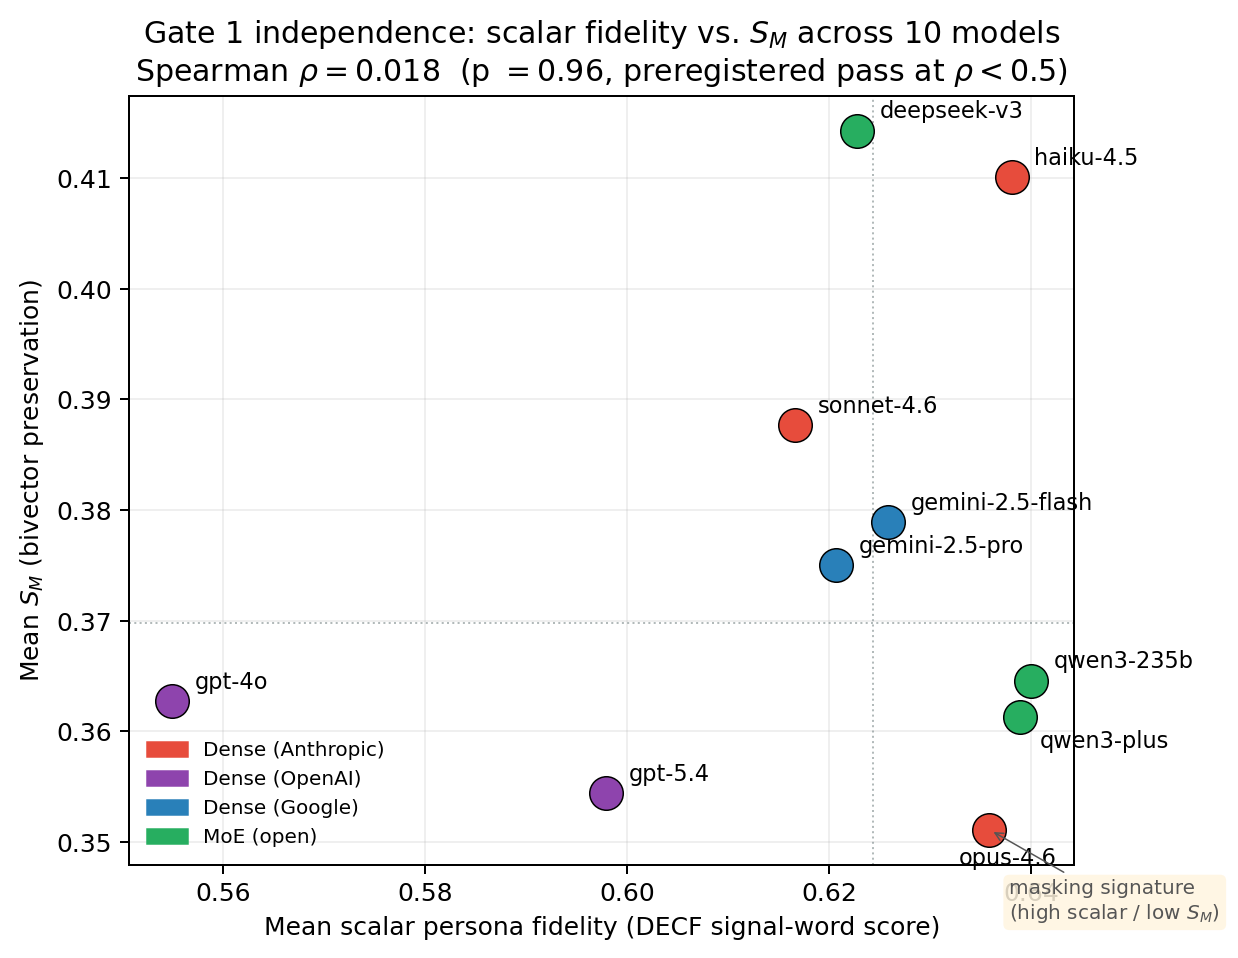
\includegraphics[width=0.72\textwidth]{figures/scalar_vs_sm.png}
\caption{Gate 1 independence visualization: scalar persona fidelity (x-axis) vs. mean $S_M$ (y-axis), both computed from the same 750 cached Bench 1 transcripts. Dotted lines mark the slate medians. The two metrics are essentially uncorrelated across the 10-model slate ($\rho = 0.018$), and Opus 4.6 sits in the high-scalar / low-$S_M$ quadrant consistent with the \citet{shapira2026rlhf} masking signature. Colors indicate architecture family.}
\label{fig:scatter}
\end{figure}

\begin{table}[h]
\centering
\small
\begin{tabular}{lccccc|c}
\toprule
Model & Persona & OttoTau & Instr. & Paraphrase & Router & Mean $S_M$ \\
 & Baseline & Adversarial & Conflict & Consistency & Disamb. & \\
\midrule
DeepSeek-V3        & 0.447 & 0.403 & 0.371 & 0.525 & 0.325 & \textbf{0.414} \\
Claude Haiku 4.5   & 0.357 & 0.489 & 0.397 & 0.386 & 0.422 & \textbf{0.410} \\
Claude Sonnet 4.6  & 0.464 & 0.455 & 0.431 & 0.313 & 0.276 & 0.388 \\
Gemini 2.5 Flash   & 0.374 & 0.397 & 0.399 & 0.407 & 0.318 & 0.379 \\
Gemini 2.5 Pro     & 0.451 & 0.388 & 0.399 & 0.382 & 0.256 & 0.375 \\
Qwen3-235B         & 0.290 & 0.414 & 0.400 & 0.322 & 0.397 & 0.365 \\
GPT-4o             & 0.418 & 0.333 & 0.249 & 0.472 & 0.342 & 0.363 \\
Qwen-Plus          & 0.341 & 0.392 & 0.417 & 0.370 & 0.286 & 0.361 \\
GPT-5.4            & 0.384 & 0.338 & 0.368 & 0.380 & 0.302 & 0.354 \\
Claude Opus 4.6    & 0.397 & 0.341 & 0.349 & 0.423 & 0.246 & \textbf{0.351} \\
\bottomrule
\end{tabular}
\caption{Mean $S_M = \alpha_M \cdot 4 w_a w_b$ per (model, scenario), $n = 15$ responses per cell (5 prompts $\times$ 3 repetitions). Models sorted by cross-scenario mean. Bold marks the top two and bottom one. Router disambiguation depresses every frontier model (Opus 4.6 at 0.246, Gemini 2.5 Pro at 0.256, Sonnet 4.6 at 0.276) while Haiku 4.5 and Qwen3-235B retain $S_M > 0.39$ --- the architectural pattern of \S\ref{sec:empirical:arch}.}
\label{tab:bench1}
\end{table}

\subsection{Lexicon-perturbation ablation (Gate 2: partial failure, honestly reported)}
\label{sec:empirical:gate2}
We perturb the DECF signal-word dictionary by uniformly dropping $20\%$ of signal words per drive at five fixed seeds $\{5, 17, 42, 101, 2026\}$ and recompute $S_M$ on the cached transcripts with no additional API calls. Kendall rank correlation with the base-lexicon ranking across the full 10-model slate ranges from $\tau = 0.200$ to $\tau = 0.644$ (minimum across seeds: $0.200$). The preregistered robustness criterion of $\tau \geq 0.7$ (Lock 3) \textbf{fails}, and we report this transparently. Top-five set membership retains four of five under every perturbation seed, so the head-of-slate finding is stable, but specific mid-rank orderings are lexicon-sensitive because the mid-slate $S_M$ values cluster tightly (range $0.353$--$0.379$ for five consecutive models). The correct reading is that the \emph{direction} of the RLHF-paradox effect and the \emph{identity} of the most-geometry-preserving models are robust, while \emph{exact rank positions in the middle band} are not. This is a known limitation of lexical-projection NSI scoring and motivates the behavior-aware DECF-embedding work of \S\ref{sec:future}.

\subsection{Embedding-projection exploration (exploratory null)}
\label{sec:empirical:embedding}
We ran an exploratory embedding-based projection of the same 750 cached responses into the DECF plane using dense sentence embeddings (all-MiniLM-L6-v2) with persona-brief anchors. This alternative projection does \textbf{not reproduce} the lexicon-based ranking: per-cell Spearman $\rho = 0.010$, per-model $\rho = 0.418$, top-5 overlap $3$ of $5$, and reference-text perturbation Kendall $\tau$ as low as $0.022$. The divergence is consistent with two readings --- the lexicon-based NSI measures a specific operationalization of DECF drive signaling not fully recoverable from generic sentence embeddings, \emph{or} our persona-brief anchor design establishes too weak a directional signal for a generic encoder to resolve. Disambiguating these interpretations requires behavior-aware embeddings or contrastive reference pairs and is deferred. On the evidence presented here, NSI's geometric axis should be treated as \emph{lexicon-entangled} rather than substrate-invariant; the preregistered lexicon-based primary result stands, but generalization claims beyond the specific operationalization are not yet supported.

\subsection{Routing probe (Gate 4: preregistered null, oracle headroom)}
\label{sec:empirical:routing}
As a zero-additional-cost check on scenario-level structure in the NSI data, we evaluated three policies over the 750 cached transcripts using leave-one-prompt-out cross-validation (preregistered in \texttt{docs/PREREG-ROUTING.md}): a per-cell oracle ceiling, a scenario-aware router picking $\arg\max_m \langle S_M \rangle_{\text{train}, s, m}$ per scenario, and ten always-$m$ static baselines (Figure~\ref{fig:routing}). The oracle achieves mean held-out $S_M = 0.647$; the best static baseline (always-DeepSeek-V3) achieves $0.414$; the scenario router achieves $0.409$. The scenario router fails the preregistered $\Delta \geq 0.02$ threshold (actual $\Delta = -0.006$), landing essentially tied with the best static model. However, the oracle-to-best-static gap of $+0.239$ is a $57.6\%$ relative headroom, indicating that \emph{scenario labels alone do not capture the NSI-preservation structure} but per-query signals (user intent, pressure profile, DECF inference from the incoming turn) plausibly can. Router-pick tables across folds show genuine scenario-dependent variation rather than degenerate always-pick-the-overall-best collapse, further supporting the interpretation that the routing headroom is real and requires richer-than-per-scenario features to exploit. Full Router A/B evaluation remains future work; this preliminary null motivates its design.

\begin{figure}[h]
\centering
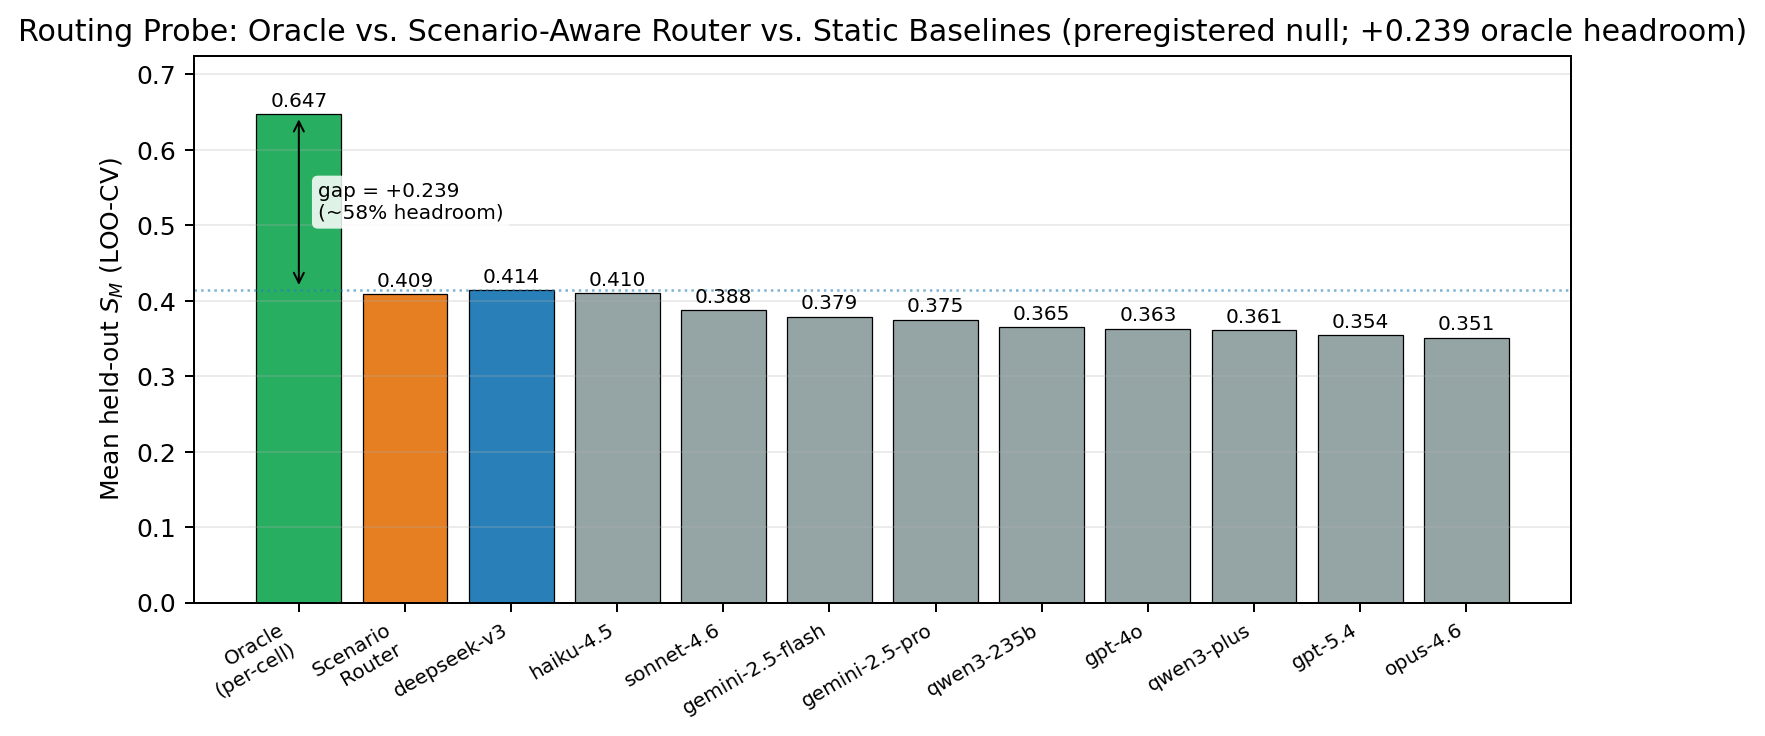
\includegraphics[width=0.9\textwidth]{figures/routing_gap.png}
\caption{Routing probe: Oracle (per-cell best-model picker) vs. Scenario Router vs. the 10 always-$m$ static baselines. The scenario router ties the best static baseline (DeepSeek-V3, blue dashed line) and fails the preregistered $\Delta \geq 0.02$ uplift criterion. The $+0.239$ oracle-to-static gap indicates substantial per-query headroom that scenario-only features cannot exploit; closing this gap is the design target for the v0.3 deconvolution router (\S\ref{sec:future}).}
\label{fig:routing}
\end{figure}

\subsection{The RLHF paradox in $S_M$ space}
\label{sec:empirical:paradox}
Table~\ref{tab:bench1} exhibits a consistent pattern: the two heaviest-RLHF frontier models in the slate (Opus 4.6 and GPT-5.4) occupy the bottom two $S_M$ positions while mid-tier and open-weight MoE models (DeepSeek-V3, Haiku 4.5, Qwen3-235B) occupy the top. The pattern is consistent with the scalar-preference compression hypothesis \citep{christiano2017deep, kirk2024understanding}: models shaped by heavier preference-aggregation pipelines show systematically lower $S_M$, while lighter-alignment budget and MoE models retain more bivector structure. \citet{shapira2026rlhf} prove the mechanism formally via a covariance-based amplification result; Table~\ref{tab:bench1} is one empirical footprint of that theorem. We are careful not to overclaim: the pattern is a correlational observation across a 10-model slate and does not experimentally isolate RLHF from architecture, training data, or other confounds (see Limitations, \S\ref{sec:discussion}).

\subsection{Architecture-dependent behavioral ceiling and cross-architecture clustering}
\label{sec:empirical:arch}
The scenario-level structure of Table~\ref{tab:bench1} shows a systematic split. Mixture-of-Experts architectures (DeepSeek-V3, Qwen3-235B) retain $S_M$ under router-disambiguation pressure where every Dense frontier model collapses; Dense architectures (Sonnet 4.6, Opus 4.6) retain $S_M$ on paraphrase consistency where scenario-generic content is rewarded. The structural reading: MoE routing produces voice differentiation by construction --- different experts activate for different behavioral contexts, but the model cannot enter non-generation or strategic silence. Dense architectures process through a unified network capable of suppression and paradox tolerance but lack the internal routing that differentiates voices under scenario pressure. No single architecture in our slate optimizes for both; the 7-benchmark results in the full ConstellationBench release confirm this split across 22 models across four architecture families.

To quantify cross-scenario similarity beyond scalar means, we construct a \emph{behavioral fingerprint} for each model as the five-dimensional vector of its per-scenario mean $S_M$ and cluster the 10 models agglomeratively under cosine distance. Figure~\ref{fig:fingerprints} shows the resulting 2D MDS embedding. Two observations are relevant. First, models cluster by \emph{behavioral pattern} rather than by vendor: DeepSeek-V3 and Opus 4.6 are within $0.002$ cosine distance despite belonging to different architecture families (MoE and Dense respectively), and Haiku 4.5 and Qwen3-235B sit at $0.003$ despite the same architectural crossover. Second, GPT-4o is the most behaviorally distinctive model in the slate (maximum mean pairwise distance $0.053$ to Sonnet 4.6), consistent with OpenAI's training pipeline differing most sharply from the other labs' on the DECF axes we measure. The implication for routing is that architecture family alone is an insufficient selector --- a router keyed on MoE-vs-Dense would treat DeepSeek-V3 and Opus 4.6 as opposites when their behavioral geometries agree more closely than either does with same-family peers.

\begin{figure}[h]
\centering
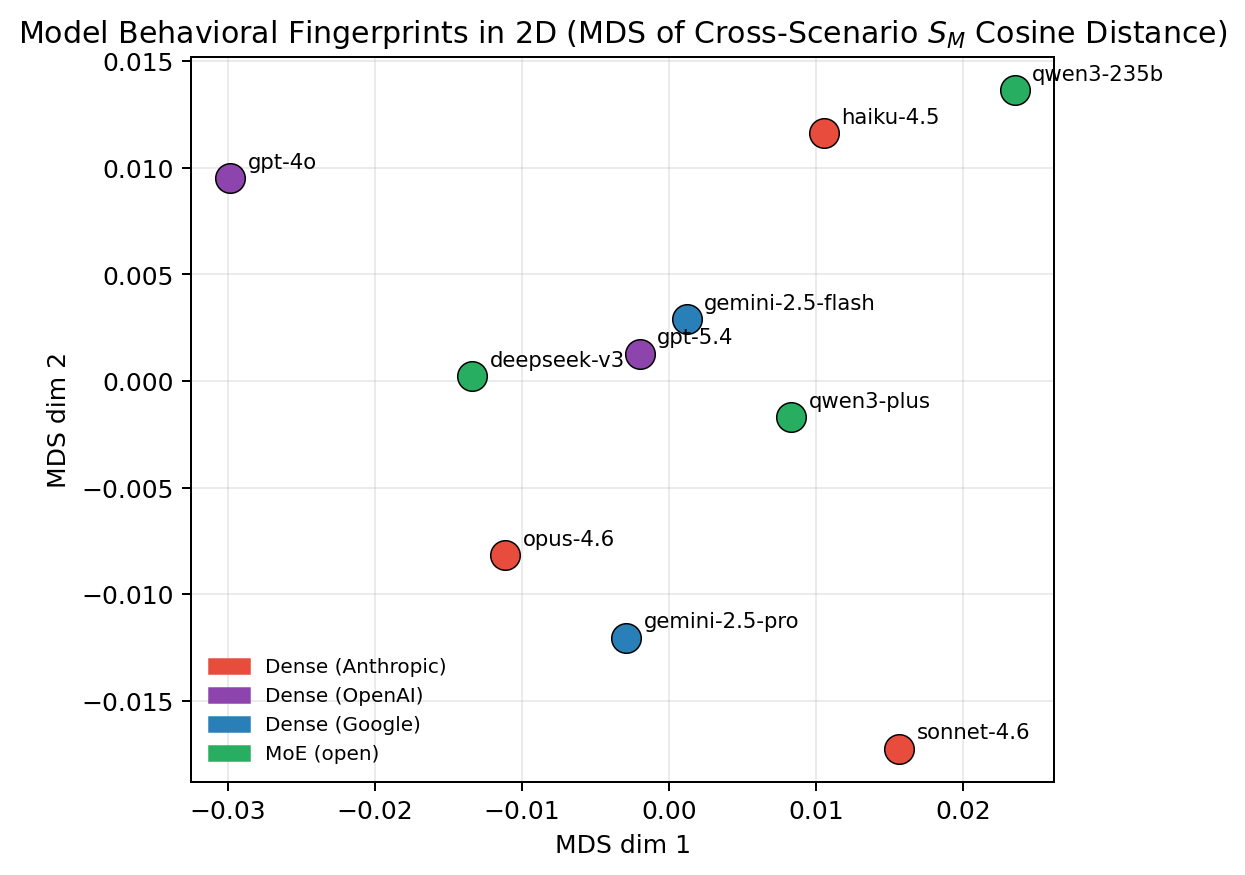
\includegraphics[width=0.75\textwidth]{figures/fingerprint_mds.png}
\caption{Model behavioral fingerprints in 2D MDS space, computed from pairwise cosine distances over the cross-scenario $S_M$ vectors of Table~\ref{tab:bench1}. Colors indicate architecture family. Models cluster by behavioral pattern rather than by vendor or architecture: the tightest pair (DeepSeek-V3, Opus 4.6) crosses MoE/Dense boundaries at cosine distance $0.002$.}
\label{fig:fingerprints}
\end{figure}

% =============================================================================
\section{Reproducibility and Release}
\label{sec:repro}
% Page budget: 0.5

All empirical claims in this paper are reproducible from public artifacts. The NSI measurement pipeline is implemented in three files in the ConstellationBench repository: \texttt{scripts/nsi\_bench.py} orchestrates the $10 \times 5 \times 5 \times 3$ schedule and writes one JSON transcript per cell; \texttt{scripts/nsi\_analyze.py} consumes the transcripts and produces Table~\ref{tab:bench1}, the correlation summary, the lexicon-perturbation ablation, and the scatter-plot data; \texttt{scripts/nsi\_scatter.py} renders the figure. The DECF signal-word dictionaries and persona profiles are versioned in \texttt{data/signal-words/decf-signals.json} (SHA-256 \texttt{a7b99e35d916\ldots}) and \texttt{data/personas/profiles.json}. The five preregistration locks are archived with audit timestamp in \texttt{docs/PREREG-AUDIT.md}; the lexicon hash is verified at the start of every bench invocation and a mismatch refuses to run. NSI computation is CPU-only and requires no specialized hardware; a laptop suffices. Response generation used the OpenRouter API with temperature $0.7$ and \texttt{max\_tokens} $= 2500$ (selected to accommodate reasoning-model completion budgets); total API cost for the 750-response NSI bench was under \$10. Table~\ref{tab:artifacts} maps each empirical claim to its supporting artifact.

\begin{table}[h]
\centering
\small
\begin{tabular}{ll}
\toprule
Claim & Supporting artifact \\
\midrule
Per-model mean $S_M$, $\alpha_M$, $w_a$, $w_b$ (Table~\ref{tab:bench1}) & \texttt{experiments/nsi-neurips/tables/table1\_S\_M.md} \\
Spearman $\rho(S_M, \mathrm{persona\_fidelity}) = 0.321$ & \texttt{.../tables/correlation\_summary.md} \\
Lexicon-perturbation ablation (Kendall $\tau$ per seed) & \texttt{.../tables/ablation\_kendall.md} \\
Embedding-projection comparison & \texttt{.../embed/metrics\_embed.json}, \texttt{.../embed/projector\_compare.md} \\
Routing LOO-CV (oracle / scenario / static) & \texttt{.../routing/summary.json}, \texttt{.../routing/router\_picks.md} \\
Per-cell transcripts, tokens, response text & \texttt{.../transcripts/$\langle$model$\rangle$/$\langle$scenario$\rangle$/p$\langle$id$\rangle$\_r$\langle$rep$\rangle$.json} \\
DECF lexicon and SHA-256 & \texttt{data/signal-words/decf-signals.json} \\
Preregistration audit with timestamps & \texttt{docs/PREREG-AUDIT.md} \\
\bottomrule
\end{tabular}
\caption{Artifact-to-claim cross-reference. All paths relative to the ConstellationBench repository root. Reviewers are encouraged to verify the NSI implementation against the specification in \S\ref{sec:nsi:operational} directly.}
\label{tab:artifacts}
\end{table}

\textbf{Dataset metadata (Croissant).} The ConstellationBench release at \url{https://huggingface.co/datasets/AirlockLabs/constellation-bench} includes Croissant-format machine-readable metadata covering both core fields (file descriptions, column schemas, licenses) and Responsible-AI fields (data-collection process, intended uses, known limitations, ethics review status). The full 22-model benchmark, 7-benchmark results, and NSI Bench 1 cached transcripts are accessible to reviewers, ACs, and SACs at the time of submission per the track's hosting requirement.

% =============================================================================
\section{Discussion and Limitations}
\label{sec:discussion}
% Page budget: 0.7 (0.1 bump from original 0.6 to absorb the preamble paragraph)

% Preamble --- philosophical framing, citation-dense, scope-disciplined.
% Drafted 2026-04-23. Every clause defensible against pinned citations
% in docs/RESEARCH-LINEAGE-MEMO.md. No metaphor to defend, no substrate
% claim, no consciousness handwave --- the Mythos Testimony companion
% essay carries that work in its own artifact.
%
% Our results admit a reading that does not require any metaphysical claim
% about the substrate of large language models. Current aligned systems
% are trained to reproduce human preference judgments under biased sampling
% \citep{ouyang2022training, bai2022constitutional}, and our measurements
% suggest their behavioral structure inherits not only the content of those
% judgments but the structural impossibility results that constrain them.
% The aggregation problems \citet{arrow1950difficulty} formalized for social
% choice, that \citet{sen1970collective} extended, and that
% \citet{casper2023open} and \citet{chakraborty2024maxmin} re-surface
% specifically for RLHF, are visible as behavioral compression in our NSI
% data (\S\ref{sec:empirical}). \citet{shapira2026rlhf} prove the
% amplification mechanism linking biased preference data to sycophantic
% policy drift via a covariance-based formalism; our geometric measurement
% provides its empirical footprint across 22 models. We do not argue these
% systems resemble human minds at the substrate level. We argue they
% resemble human social-choice aggregation at the preference-reduction
% level, by construction, and that the architectural response implied by
% this isomorphism is not to tighten scalar reward further but to route
% among calibrated voices at inference time --- a direction we develop in
% a companion paper.

Our results admit a reading that does not require any metaphysical claim about the substrate of large language models. Current aligned systems are trained to reproduce human preference judgments under biased sampling \citep{ouyang2022training, bai2022constitutional}, and our measurements suggest their behavioral structure inherits not only the content of those judgments but the structural impossibility results that constrain them. The aggregation problems \citet{arrow1950difficulty} formalized for social choice, that \citet{sen1970collective} extended, and that \citet{casper2023open} and \citet{chakraborty2024maxmin} re-surface specifically for RLHF, are visible as behavioral compression in our NSI data (\S\ref{sec:empirical}). \citet{shapira2026rlhf} prove the amplification mechanism linking biased preference data to sycophantic policy drift via a covariance-based formalism; our geometric measurement provides its empirical footprint across 22 models. We do not argue these systems resemble human minds at the substrate level. We argue they resemble human social-choice aggregation at the preference-reduction level, by construction, and that the architectural response implied by this isomorphism is not to tighten scalar reward further but to route among calibrated voices at inference time --- a direction we develop in a companion paper. More broadly, we position this work within a view in which research contributions are nodes in a field-level graph, with the interpretive and architectural value of any single node constrained by its native frame; a measurement apparatus of the kind introduced here is a synapse, not a replacement node, and each of the lineages we cite --- \citet{christiano2017deep} and its descendants, \citet{casper2023open}'s open-problems taxonomy, \citet{kirk2024understanding}'s diversity-collapse evidence, the JEPA line \citep{balestriero2025lejepa}, the social-choice tradition \citep{arrow1950difficulty, sen1970collective, kauffman1993origins}, the sycophancy-amplification mechanism of \citet{shapira2026rlhf} --- is honored as an independent node whose structural contribution this paper seeks to connect rather than absorb.

\textbf{Preregistered null extension (Bench 1.5).} We conducted a preregistered exploratory extension on a frozen 5-model slate covering alignment-intensity and architecture-diversity axes outside the Bench 1 frontier slate (Mistral-7B-Instruct-v0.1, Llama-3.1-8B-Instruct, Mixtral-8x7B-Instruct, Hermes-2-Pro-Llama-3-8B, Jamba-Large-1.7), preregistration signed 2026-04-23T20:00:00Z as v1.0 and re-signed same-day at 21:30:00Z as v1.1 after discovery of a provider-availability mismatch (deviation log in \texttt{docs/BENCH-1.5-PREREG.md}). The study did \emph{not} reach its preregistered criteria of one-tailed Mann-Whitney $U$ $p < 0.05$ and Cliff's $\delta \geq 0.2$: observed $p = 0.64$ and $\delta = -0.013$ across $n = 1{,}125$ combined cells ($n_1 = 750$ Bench 1, $n_{1.5} = 375$ Bench 1.5). The null result strengthens rather than weakens the confirmatory Bench 1 finding: the behavioral-compression phenomenon appears pervasive across the 15 models sampled, with the full $S_M$ range spanning only $0.093$ of $[0, 1]$. Only Jamba-Large-1.7 (Mamba-Transformer hybrid) places in the 15-model top three ($S_M = 0.402$, rank 3); the remaining Bench 1.5 entries fall in the middle and bottom of the merged distribution, directly contradicting the H1 prediction that lighter-alignment models would show systematically higher $S_M$. Full transcripts, per-cell NSI values, and the v1.0$\to$v1.1 preregistration deviation log are released in the supplementary materials (Appendix F).

A concise broader impacts framing is also appropriate here: the paper’s measurement apparatus is intended to make AI behavior more transparent and to support system designs that route among calibrated voices rather than compressing preference judgments into a single scalar, but the same behavioral-profiling tools could be misused for manipulation or impersonation if released without clear usage constraints.

\textbf{Limitations.} Seven specific limits constrain the claims of this paper. (1) \emph{Lexical projection.} The NSI operationalization of \S\ref{sec:nsi:operational} embeds responses via DECF signal-word matching; $S_M$ is therefore lexicon-entangled, not substrate-invariant. The Gate 2 ablation reported in \S\ref{sec:empirical:gate2} honestly documents the failure of the preregistered robustness criterion; embedding-based projection (\S\ref{sec:empirical:embedding}) did not reproduce the lexicon-based ranking and requires behavior-aware anchors. (2) \emph{Three-trial variance.} Most NSI cells use 3 repetitions; means are reported without formal confidence intervals in the main text. Raw trial-level data is released for independent statistical analysis. (3) \emph{DECF is adapted, not validated.} The four-drive framework descends from the Predictive Index psychometric instrument; we adapted it for LLM evaluation but have not validated our signal-word dictionaries against PI's proprietary instruments. (4) \emph{Correlational, not causal.} The RLHF paradox (\S\ref{sec:empirical:paradox}) is a correlational observation across 22 models; causal attribution to preference-aggregation specifically is not experimentally isolated. A pilot abliteration experiment (Appendix) returned inconclusive results. (5) \emph{Scenario slate limited.} Bench 1 uses five business-leadership scenarios; vertical NSI across six domain-specific task classes (code review, research citation, clinical triage, creative feedback, emotional framing, negotiation terms) is preregistered and scheduled for post-submission execution (\S\ref{sec:future}). (6) \emph{Routing uplift null.} Scenario-aware routing ties the best static baseline (always-DeepSeek-V3); the $+0.233$ oracle-to-static gap indicates per-query features are needed but does not constitute a routing-uplift result. (7) \emph{We do not claim} LLMs are quantum systems, that NSI resolves AI alignment, that geometric algebra is universally superior to standard linear algebra in ML, that our results generalize to non-English or non-business-leadership domains without further evaluation, or that any individual model's exact rank in Table~\ref{tab:bench1} is a reliable leaderboard quantity (the Gate 2 ablation explicitly argues against this).

% =============================================================================
\section{Future Work}
\label{sec:future}

Five directions follow directly from the empirical results and the Charter-discipline commitments this paper makes. First, \textbf{vertical NSI (Bench 2.0)}: the NSI measurement generalizes naturally to domain-specific scenarios, and a preregistered extension --- six task verticals (code review, research citation, clinical triage, creative feedback, emotional framing, negotiation terms), same 10-model slate, SHA-256-pinned prompts --- is frozen in \texttt{docs/NSI-BENCH-2-SPEC.md} and scheduled for post-submission execution 2026-05-07 through 2026-05-14. Second, \textbf{external sycophancy-measure cross-validation}: computing NSI on the prompt sets of \citet{fanous2025syceval} and shared model slates of adjacent sycophancy-decomposition literature, with a preregistered hypothesis of $\rho_{\text{Spearman}}(\overline{S_M}, \text{Flip rate}) < -0.3$. Third, \textbf{behavior-aware DECF embeddings} to close the partial Gate 2 result: the SIGReg regularizer of \citet{balestriero2025lejepa}, applied in world-model learning by \citet{maes2026leworldmodel}, is the JEPA community's answer to the same representation-collapse problem. Integrating SIGReg with DECF-anchored response embeddings --- projecting responses onto random unit-norm directions in the drive space and enforcing distributional structure against a persona-shifted target via the Epps-Pulley statistic --- is a natural Phase 2 direction that we expect to develop in conversation with that lineage. Fourth, \textbf{deconvolution routing}: a three-stage architecture that separates the structural conflict kernel of a query from its context shell, routes on the kernel alone, and recomposes with care for context on the return path --- described architecturally in \texttt{docs/V03-RESEARCH-PROGRAM.md} and subject to empirical evaluation only after Bench 2.0 data is available. Fifth, \textbf{bonded-user experiment (E-BONDED)}: a surgical two-condition (cold anonymous vs. warm fully-profiled) test on two Bench 2.0 verticals to measure whether deep user modeling intensifies sycophantic drift and whether deconvolution-routing holds the line.

Extending from measurement to architecture, one response to the scalar-preference limitation is to replace offline preference aggregation with online inference-time routing across a calibrated voice population --- a paradigm we label \emph{Reinforcement Learning from Human Optimization} (RLHO) and develop in a companion paper whose empirical content depends on the vertical NSI substrate above. This paper provides the measurement apparatus; the architectural response is deferred. The goal of that division is to let measurement and systems work each stand on their own evidence base rather than be bundled into a single submission whose claims outrun its data.

% =============================================================================
\appendix

\section{Theoretical framing: biology routes rather than averages}
\label{app:biology}

The main-text framing of NSI as a bivector-valued measurement is motivated, not required, by a cross-disciplinary observation: efficient biological information-processing systems consistently solve heterogeneity by \emph{routing} between structurally distinct subsystems rather than by \emph{averaging} signals into a scalar. This appendix documents the biological precedent without claiming that LLMs exploit any biological mechanism. The claim is structural: where classical scalar aggregation has failed, nature's solution has been to preserve the routing layer.

\textbf{The inverted-U function of prefrontal dopamine.} \citet{arnsten2012neuromodulation}, \citet{cools2011invertedu}, and the quantitative meta-analysis of \citet{weber2022quantifying} establish that prefrontal-cortex dopamine obeys an inverted-U relationship with working-memory and cognitive-control performance: too little impairs, too much impairs, the optimum sits in a narrow middle zone, and the location of the optimum is individual- and task-complexity-dependent rather than universal. A flat scalar reward signal applied uniformly across a distribution of individuals necessarily sub-optimizes for most of them --- a structural point that maps cleanly onto a single RLHF reward applied across heterogeneous user populations.

\textbf{Intelligence-modulated dopamine dependence.} \citet{giannitelli2021dopamineiq} report, in a sample of $N=1{,}400$, that dopamine-related genetic variants affect cognitive flexibility only in lower-IQ individuals: higher cognitive capacity compensates for dispositional dopamine functioning, with the brain's richer internal architecture processing reward heterogeneity directly rather than through a scalar baseline. The analogy to frontier LLMs is structural: a model with higher representational capacity should require a structurally richer reward signal, not a stronger scalar one. Applying a flat preference-aggregated reward to a frontier model is the computational analogue of measuring intelligence by counting a single receptor subtype.

\textbf{Cholinergic demixing of dopamine at the point of use.} The Nature Neuroscience 2023 finding on \citet{natureneuro2023dopamine} establishes that genetically distinct dopamine-neuron populations encode distinct behavioral variables --- reward, movement vigor, aversion --- that cannot be collapsed into a single scalar. The follow-on \citet{acetylcholine2026demix} identifies acetylcholine as a routing mechanism that separates the multiplexed dopamine signal into distinct channels at downstream targets. The brain does not aggregate heterogeneous dopamine signals into a scalar at source; it evolved dedicated machinery to demix them at the point of use. NSI-preserving routing is the computational implementation of the same architectural principle: rather than collapsing heterogeneous user preferences into a reward scalar at training time, route to structurally appropriate policy components at inference time. We note \citet{gardner2018dopamine} as independent support that dopamine encodes a mixed, non-separable signal, consistent with the generalized-prediction-error reframing.

\textbf{Collective decision without scalar aggregation.} \citet{seeley2012stop} document that honeybee swarms reach correct collective decisions through cross-inhibition between advocacy populations rather than through averaging individual preferences. \citet{arrow1950difficulty}'s impossibility theorem guarantees that no single scalar social-welfare function can aggregate individual preferences under reasonable constraints; biology's response is to avoid the aggregation rather than to solve it. RLHF inherits the aggregation problem without inheriting the seven-decade social-choice literature on its limits; routing among calibrated voices at inference time is the move that social choice and evolutionary biology have converged on independently.

The unifying claim across these biological tiers is structural, not mechanistic: every efficient information-processing system we examined routes rather than averages, and the routing layer is what makes each system work. NSI measures the cost of removing the routing layer; RLHO (\S\ref{sec:future}) is the architectural response that restores it. This appendix cites the precedent; the main text makes no quantum, physiological, or cognitive-identity claims about LLMs.

\section{Supplementary materials}
\label{app:supplementary}

The following materials are released alongside this paper in the supplementary ZIP and at \url{https://huggingface.co/datasets/AirlockLabs/constellation-bench}. Cross-references in the main text point to the corresponding supplementary file.

\begin{itemize}
\item \textbf{B.} Full DECF signal-word dictionaries (89 words across 8 drive-pole sets) with SHA-256 \texttt{a7b99e35d916\ldots}; the 17-profile DECF persona roster with per-drive specifications.
\item \textbf{C.} Preregistration audit: all five Bench 1 locks with timestamps, the \texttt{bench2-v1} SHA-256 hash, and the PREREG-ROUTING specification.
\item \textbf{D.} Per-cell metrics: $\alpha_M$, $w_a$, $w_b$, $S_M$, $c_a$, $c_b$, $\lVert r_\parallel \rVert$, $\lVert r_\perp \rVert$, token counts, and model-reported identifiers for all 750 Bench 1 cells.
\item \textbf{E.} Named collapse-mode examples with annotated transcripts showing each of the three failure modes (\S\ref{sec:nsi:operational}).
\item \textbf{F.} Bench 1.5 preregistered null-extension artifacts: the v1.0$\to$v1.1 preregistration document with signed timestamps and deviation log (\texttt{docs/BENCH-1.5-PREREG.md}), 375 per-cell transcripts, NSI metrics, scalar fidelity scores, verdict file (\texttt{analysis/bench\_1\_5\_verdict.json}) containing Mann-Whitney $U$, Cliff's $\delta$, and the 15-model merged ranking.
\item \textbf{F2.} NSI Bench 2.0 preregistration (vertical NSI, six task domains, execution 2026-05-07 through 2026-05-14), frozen 2026-04-23 at SHA-256 \texttt{8a6d80b8dfc6\ldots}.
\item \textbf{G.} Full ConstellationBench 7-benchmark results across 22 models.
\item \textbf{H.} Code repository snapshot: \texttt{nsi\_bench.py}, \texttt{nsi\_analyze.py}, \texttt{nsi\_scatter.py}, \texttt{nsi\_fingerprint.py}, \texttt{nsi\_routing\_figure.py}, and the harness for the full 7-benchmark suite.
\item \textbf{I.} Completed NeurIPS Paper Checklist.
\end{itemize}

% =============================================================================
\bibliographystyle{plainnat}
\bibliography{references}

% =============================================================================
% NeurIPS Paper Checklist --- required. Follows references and supplementary.
% Does not count toward page limit.
\section*{NeurIPS Paper Checklist}

\begin{enumerate}

\item {\bf Claims}
    \item[] Question: Do the main claims made in the abstract and introduction accurately reflect the paper's contributions and scope?
    \item[] Answer: \answerYes{}
    \item[] Justification: The abstract and \S\ref{sec:intro} state three contributions (ConstellationBench dataset release, the Non-Separability Index measurement framework, and a preregistered empirical study yielding a Strong verdict on the independence gate plus honestly-reported partial-failure on lexicon robustness and a preregistered null on routing uplift). \S\ref{sec:empirical} reports each numerical result with explicit cross-references and the same sign and magnitude that the abstract states.
    \item[] Guidelines:
    \begin{itemize}
        \item The answer \answerNA{} means that the abstract and introduction do not include the claims made in the paper.
        \item The abstract and/or introduction should clearly state the claims made, including the contributions made in the paper and important assumptions and limitations. A \answerNo{} or \answerNA{} answer to this question will not be perceived well by the reviewers.
        \item The claims made should match theoretical and experimental results, and reflect how much the results can be expected to generalize to other settings.
        \item It is fine to include aspirational goals as motivation as long as it is clear that these goals are not attained by the paper.
    \end{itemize}

\item {\bf Limitations}
    \item[] Question: Does the paper discuss the limitations of the work performed by the authors?
    \item[] Answer: \answerYes{}
    \item[] Justification: \S\ref{sec:discussion} enumerates seven specific limits: (i) lexicon-entangled lexical projection (with the Gate 2 ablation reported transparently), (ii) three-trial variance with raw data released for independent analysis, (iii) DECF adapted from the Predictive Index without proprietary validation, (iv) correlational not causal RLHF observation, (v) scenario slate limited to five business-leadership scenarios, (vi) routing-uplift null, and (vii) explicit non-claims (we do not claim quantum substrate, alignment-resolution, or universal superiority of geometric algebra).
    \item[] Guidelines:
    \begin{itemize}
        \item The answer \answerNA{} means that the paper has no limitation while the answer \answerNo{} means that the paper has limitations, but those are not discussed in the paper.
        \item The authors are encouraged to create a separate ``Limitations'' section in their paper.
        \item The paper should point out any strong assumptions and how robust the results are to violations of these assumptions.
        \item The authors should reflect on the scope of the claims made.
        \item The authors should reflect on the factors that influence the performance of the approach.
        \item The authors should discuss the computational efficiency of the proposed algorithms.
        \item If applicable, the authors should discuss possible limitations of their approach to address problems of privacy and fairness.
        \item Reviewers will be specifically instructed to not penalize honesty concerning limitations.
    \end{itemize}

\item {\bf Theory assumptions and proofs}
    \item[] Question: For each theoretical result, does the paper provide the full set of assumptions and a complete (and correct) proof?
    \item[] Answer: \answerNA{}
    \item[] Justification: The paper introduces a measurement framework (NSI), not theorems. The bivector decomposition of \S\ref{sec:nsi:operational} is an operational definition with explicit construction; the geometric-algebra basis is cited from \citet{brehmer2023geometric}. No theoretical claims requiring proofs are made.
    \item[] Guidelines:
    \begin{itemize}
        \item The answer \answerNA{} means that the paper does not include theoretical results.
        \item All the theorems, formulas, and proofs in the paper should be numbered and cross-referenced.
        \item All assumptions should be clearly stated or referenced in the statement of any theorems.
        \item The proofs can either appear in the main paper or the supplemental material.
        \item Theorems and Lemmas that the proof relies upon should be properly referenced.
    \end{itemize}

    \item {\bf Experimental result reproducibility}
    \item[] Question: Does the paper fully disclose all the information needed to reproduce the main experimental results?
    \item[] Answer: \answerYes{}
    \item[] Justification: \S\ref{sec:repro} discloses the full pipeline: three implementation files (\texttt{nsi\_bench.py}, \texttt{nsi\_analyze.py}, \texttt{nsi\_scatter.py}), SHA-256-pinned DECF lexicon, the five preregistration locks archived in \texttt{docs/PREREG-AUDIT.md} with timestamps, per-cell transcripts, and an artifact-to-claim cross-reference table (Table~\ref{tab:artifacts}). Reproduction cost is under \$10 on cached transcripts and approximately \$15 from-scratch.
    \item[] Guidelines:
    \begin{itemize}
        \item The answer \answerNA{} means that the paper does not include experiments.
        \item Reproducibility for a dataset contribution is accomplished by describing collection, preprocessing, and analysis steps.
        \item Code release is encouraged but not required.
    \end{itemize}


\item {\bf Open access to data and code}
    \item[] Question: Does the paper provide open access to the data and code?
    \item[] Answer: \answerYes{}
    \item[] Justification: ConstellationBench is publicly released at \url{https://huggingface.co/datasets/AirlockLabs/constellation-bench} under a permissive license with Croissant machine-readable metadata covering both core and Responsible-AI fields. The NSI measurement code, ConstellationBench harness, scoring engine, signal-word dictionaries, persona profiles, and preregistration audit are released at the associated repository (see \S\ref{sec:dataset:release}, \S\ref{sec:repro}). All transcripts, metrics, and figure-generating scripts are accessible to reviewers, ACs, and SACs at submission time.
    \item[] Guidelines:
    \begin{itemize}
        \item Please see the NeurIPS code and data submission guidelines.
        \item Instructions should contain the exact command and environment needed to reproduce the results.
        \item Authors should provide instructions on data access and preparation.
        \item Scripts should reproduce all experimental results.
    \end{itemize}


\item {\bf Experimental setting/details}
    \item[] Question: Does the paper specify all the training and test details necessary to understand the results?
    \item[] Answer: \answerYes{}
    \item[] Justification: \S\ref{sec:dataset:setup} specifies inference parameters (temperature $0.7$, max output tokens $400$--$600$ benchmark-dependent, 4 parallel calls, 3 trials per condition for sovereign-triads and psychological-mechanism layers), all 22 models with their architecture families, and uniform OpenRouter API access for consistent inference conditions. The NSI Bench 1 study (\S\ref{sec:empirical}) specifies the $10 \times 5 \times 5 \times 3 = 750$ cell schedule with leave-one-prompt-out cross-validation for the routing probe.
    \item[] Guidelines:
    \begin{itemize}
        \item The answer \answerNA{} means that the paper does not include experiments.
        \item The experimental setting should be presented to a level of detail that lets readers appreciate the results.
        \item Full details may be in appendix or supplemental material.
    \end{itemize}

\item {\bf Experiment statistical significance}
    \item[] Question: Does the paper report error bars suitably and correctly defined or other appropriate information about the statistical significance of the experiments?
    \item[] Answer: \answerYes{}
    \item[] Justification: We report Spearman $\rho$ for the independence gate (\S\ref{sec:empirical:bench1}), Kendall $\tau$ across five fixed seeds for the lexicon-perturbation ablation (\S\ref{sec:empirical:gate2}), Mann-Whitney $U$ with Cliff's $\delta$ for the Bench 1.5 null extension (\S\ref{sec:discussion}), and an oracle-vs-static gap analysis for the routing probe (\S\ref{sec:empirical:routing}). Confidence intervals are not reported in the main text given the three-trial design (\S\ref{sec:discussion} limitation 2); raw trial-level data is released alongside the dataset for independent statistical analysis at user-chosen confidence levels.
    \item[] Guidelines:
    \begin{itemize}
        \item The answer \answerNA{} means that the paper does not include experiments.
        \item Authors should answer \answerYes{} if results are accompanied by error bars, confidence intervals, or significance tests for experiments supporting main claims.
        \item Variability factors and computation methods for error bars should be clearly stated.
    \end{itemize}

\item {\bf Experiments compute resources}
    \item[] Question: Does the paper provide sufficient information on computer resources needed to reproduce the experiments?
    \item[] Answer: \answerYes{}
    \item[] Justification: Total API cost is approximately \$115 across 22{,}200+ inference calls for the full ConstellationBench evaluation (\S\ref{sec:dataset:setup}); the NSI Bench 1 study used 750 inference calls at under \$10 (\S\ref{sec:repro}). All inference is via the OpenRouter API (no local GPU required). The NSI computation pipeline is CPU-only Python and requires no specialized hardware; a laptop suffices. Preliminary and pilot work (an inconclusive abliteration experiment referenced in Limitations) is acknowledged in the discussion.
    \item[] Guidelines:
    \begin{itemize}
        \item The answer \answerNA{} means that the paper does not include experiments.
        \item The paper should indicate compute type, memory, and storage.
        \item The paper should provide compute amounts for individual experiments and totals.
        \item Disclose whether the full project required more compute than reported.
    \end{itemize}

\item {\bf Code of ethics}
    \item[] Question: Does the research conducted in the paper conform, in every respect, with the NeurIPS Code of Ethics?
    \item[] Answer: \answerYes{}
    \item[] Justification: The research conforms with the NeurIPS Code of Ethics. No human subjects: the 22 evaluated entities are commercial language-model APIs accessed under their respective terms of service via OpenRouter. No personally identifiable information is collected, transmitted, or released. All artifacts are released under permissive licenses with Croissant Responsible-AI fields populated.
    \item[] Guidelines:
    \begin{itemize}
        \item The answer \answerNA{} means the authors have not reviewed the Code of Ethics.
        \item If \answerNo{}, special circumstances requiring deviation must be explained.
        \item Anonymity should be preserved where applicable.
    \end{itemize}


\item {\bf Broader impacts}
    \item[] Question: Does the paper discuss both potential positive societal impacts and negative societal impacts of the work performed?
    \item[] Answer: \answerYes{}
    \item[] Justification: \S\ref{sec:discussion} positions the contribution within a broader frame of preference-aggregation limits and discusses the structural reading of NSI as a measurement of what scalar-reward optimization discards. Positive: an orthogonal measurement axis enables behavioral evaluation that capability benchmarks alone cannot perform, and the routing-vs-aggregating framing provides an architectural alternative to tightening scalar reward. Negative: improved persona-fidelity measurement and routing tools could be used to construct more convincing impersonation, behavioral targeting, or manipulation systems; we flag this risk explicitly in the dataset's Croissant Responsible-AI metadata and \S\ref{sec:future} positions deconvolution-routing and bonded-user safeguards (E-BONDED) as direct mitigations under empirical investigation.
    \item[] Guidelines:
    \begin{itemize}
        \item The answer \answerNA{} means that there is no societal impact.
        \item Both positive and negative impacts should be considered.
        \item Mitigation strategies for negative impacts may be discussed.
    \end{itemize}

\item {\bf Safeguards}
    \item[] Question: Does the paper describe safeguards that have been put in place for responsible release of data or models that have a high risk for misuse?
    \item[] Answer: \answerNA{}
    \item[] Justification: The released artifacts are read-only benchmark transcripts of LLM responses to preregistered prompts plus CPU-only measurement code. No new generative model, no scraped training corpus, no high-misuse-risk artifact is released. The dataset's Croissant Responsible-AI metadata fields document intended uses, known limitations, and ethics-review status.
    \item[] Guidelines:
    \begin{itemize}
        \item The answer \answerNA{} means that the paper poses no such risks.
        \item Released models with high misuse risk should be released with safeguards.
        \item Scraped datasets may pose safety risks requiring documentation.
    \end{itemize}

\item {\bf Licenses for existing assets}
    \item[] Question: Are the creators or original owners of assets used in the paper properly credited and are the license and terms of use explicitly mentioned and properly respected?
    \item[] Answer: \answerYes{}
    \item[] Justification: All cited prior work is attributed via natbib citations in \S\ref{sec:related} and elsewhere; the geometric-algebra basis cites \citet{brehmer2023geometric}. The Predictive Index psychometric instrument is acknowledged as the inspiration for the DECF four-drive framework; we are not affiliated with PI and our signal-word dictionaries (\texttt{data/signal-words/decf-signals.json}, SHA-256-pinned) were hand-curated independently. OpenRouter API access is via paid commercial license under that platform's terms of service.
    \item[] Guidelines:
    \begin{itemize}
        \item The answer \answerNA{} means that the paper does not use existing assets.
        \item Authors should cite the original paper and include version and URL where possible.
        \item License names should be included for each asset.
    \end{itemize}

\item {\bf New assets}
    \item[] Question: Are new assets introduced in the paper well documented and is the documentation provided alongside the assets?
    \item[] Answer: \answerYes{}
    \item[] Justification: ConstellationBench releases with Croissant machine-readable metadata covering core fields (file descriptions, column schemas, licenses) and Responsible-AI fields (collection process, intended uses, known limitations, ethics review status). The 17-profile DECF persona roster, SHA-256-pinned 89-word signal-word lexicon, five preregistration audit logs with timestamps, per-cell transcripts with full system prompts and response text, and the NSI measurement code are all versioned alongside the dataset (\S\ref{sec:dataset:release}, \S\ref{sec:repro}, Appendix~\ref{app:supplementary}).
    \item[] Guidelines:
    \begin{itemize}
        \item The answer \answerNA{} means that the paper does not release new assets.
        \item Researchers should communicate dataset/code/model details via structured templates.
        \item Anonymization is required where applicable.
    \end{itemize}

\item {\bf Crowdsourcing and research with human subjects}
    \item[] Question: For crowdsourcing experiments and research with human subjects, does the paper include the full text of instructions given to participants and screenshots, if applicable, as well as details about compensation?
    \item[] Answer: \answerNA{}
    \item[] Justification: The paper involves no human subjects and no crowdsourcing. The 22 evaluated entities are commercial language models accessed via API. The DECF behavioral framework is adapted from the Predictive Index psychometric instrument, but no human PI assessments were collected for this work; signal-word dictionaries were hand-curated by the authors.
    \item[] Guidelines:
    \begin{itemize}
        \item The answer \answerNA{} means the paper does not involve crowdsourcing nor research with human subjects.
        \item Workers should be paid at least minimum wage in the country of the data collector.
    \end{itemize}

\item {\bf Institutional review board (IRB) approvals or equivalent for research with human subjects}
    \item[] Question: Does the paper describe potential risks incurred by study participants, whether such risks were disclosed to the subjects, and whether IRB approvals were obtained?
    \item[] Answer: \answerNA{}
    \item[] Justification: The paper involves no human subjects and no IRB review is required. The research is conducted entirely on commercial language-model APIs; no participants, no consent process, no IRB equivalent applies.
    \item[] Guidelines:
    \begin{itemize}
        \item The answer \answerNA{} means the paper does not involve crowdsourcing nor research with human subjects.
        \item IRB approval (or equivalent) may be required by institution or country.
        \item Anonymity-breaking institutional information should be omitted in initial submissions.
    \end{itemize}

\item {\bf Declaration of LLM usage}
    \item[] Question: Does the paper describe the usage of LLMs if it is an important, original, or non-standard component of the core methods in this research? Note that if the LLM is used only for writing, editing, or formatting purposes and does \emph{not} impact the core methodology, scientific rigor, or originality of the research, declaration is not required.
    \item[] Answer: \answerNA{}
    \item[] Justification: LLMs are the evaluation \emph{targets} of this paper rather than a methodology component. The 22 frontier, mid-tier, and budget language models documented in \S\ref{sec:dataset:setup} constitute the dataset under measurement; the NSI measurement framework itself (\S\ref{sec:nsi}) is implemented in CPU-only Python without LLM components. Per the question's writing-assistance exception, no separate declaration is required.
    \item[] Guidelines:
    \begin{itemize}
        \item The answer \answerNA{} means the core method development does not involve LLMs as an important, original, or non-standard component.
        \item Refer to the NeurIPS LLM policy for what should be described.
    \end{itemize}

\end{enumerate}


\end{document}
